\graphicspath{{snoga/}}
\chapter{Evolutionary Multi-objective Optimization Improves Phylogenomic Analysis}



	Species tree estimation from multi-locus data is complicated as biological processes can result in different loci having different evolutionary histories. Incomplete lineage sorting (ILS), modeled by the multi-species coalescent (MSC), is considered to be a dominant cause for gene tree incongruence. Various optimization criteria (e.g., quartet score, pseudo-likelihood, etc.) are statistically consistent under the MSC model, meaning that they return the true species tree with high probability given sufficiently large numbers of accurate gene trees. However, the number of genes is limited and estimating highly accurate gene trees is difficult. Therefore, even the statistically consistent methods may fail to reconstruct highly accurate trees under practical model conditions with limited numbers of genes and in the presence of gene tree estimation error. In this paper, we present an evolutionary multi-objective optimization (EMO) algorithm (SNOGA), a modified version of the popular NSGAII, which combines various optimization criteria to find a suitable search space containing highly accurate species trees. Our experimental results on a collection of simulated datasets demonstrate that the EMO approach can lead us to a tree-space containing significantly better trees than the trees estimated by ASTRAL and MP-EST which are two of the most widely used methods. 

 \section{Introduction}
\label{sec:intro}
In biological studies, phylogeny refers to the evolutionary relationships/history among a set of entities such as species, genes, etc. The entities under consideration are generally referred to as taxa. Each such taxon is placed as a leaf in a phylogenetic tree and the tree topology represents the evolutionary history. The non-leaf (i.e. internal) nodes of the tree represent hypothetical ancestral taxa from which the present day taxa evolved. These ancestral taxa are believed to have existed in the past, but has become extinct. Notably, a tree $T$ is a connected acyclic graph with a set of vertices $V$ and a set of edges $E$. An edge $e = (u, v) \in E$ represents an evolutionary relationship between the two taxa represented by the vertices $u$ and $v$. Knowledge discovered through analyzing such trees has benefited several branches of science including but not limited to medicine, forensics, bio-geography, epidemiology~\cite{felix2015phylogenetics}. 
Fig.~\ref{fig:outgroup} shows a sample phylogenetic tree among four species: human, chimpanzee, gorilla and orangutan. This evolutionary tree depicts that human and chimpanzee share a common ancestor. As such, we consider humans to be more closely related to chimpanzees than they are to gorillas and orangutans.

\begin{figure}[!tb]
	\centering
	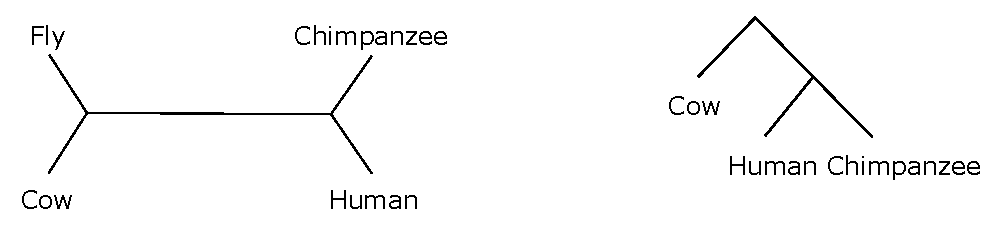
\includegraphics[width=0.5\textwidth]{Figure/outgroup.eps}
	\caption{A phylogenetic tree relating four species: human, chimpanzee, gorilla and orangutan. }
	\label{fig:outgroup}
\end{figure}




A species tree represents the evolutionary relationships of a group of organisms. On the other hand, the phylogeny specific to a particular region of the genome (known as locus or gene) is termed as a gene tree~\cite{maddison1997gene}. These concepts will be discussed shortly
in a subsequent section. In this study, we tackle the problem of inferring the species tree using evolutionary multi-objective optimization (EMO) approach. An EMO algorithm evolves a population (i.e., a set of candidate solutions) by simultaneously optimizing multiple criteria end eventually outputs a collection of candidate solutions. In this paper, we focus on finding a tree-space by an EMO algorithm containing highly accurate trees under practical model conditions with limited numbers of estimated gene trees. Our main contributions can be summarized as follows.

\begin{itemize}
	\item To the best of our knowledge, for the first
	time we address the task of species tree estimation as a multi-objective optimization problem (MOP) by simultaneously optimizing three objectives. 
	
	\item We adapt NSGAII, a popular Pareto domination based EMO algorithm, by integrating problem-specific operators for this task. More importantly, we design a specially customized algorithm, namely, SNOGA, by modifying NSGAII.
	
	\item We investigated whether a Pareto domination based EMO algorithm is appropriate for this task by examining the operations of NSGAII and SNOGA on a collection of challenging simulated datasets. This reveals 
	
	\item We assess the validity of our approach by comparing its performance with widely used existing methods. Our results suggest that the EMO approach can produce a tree-space that contains substantially more accurate trees than the trees estimated by optimizing the individual criterion.
\end{itemize}

The rest of the paper is organized as follows. Related works
are discussed in Section 2. Preliminaries and formulation
of the multi-objective species tree estimation problem are presented in Section 3. Section 4 introduces the chosen EMO algorithms. Experimental
results examining the proposed approach along with comparative analysis are provided in Section 5. Finally, Section 6 presents
conclusions and future extension of this study.





\section{Related Works}
A standard approach for species tree estimation uses multiple loci, then concatenates alignments for each locus
into a super-matrix based on the assumption that all genes have the same gene tree topology~\cite{huelsenbeck1996combining, de2007supermatrix}, which is then used to estimate a species phylogeny. When all the genes evolve down the same tree topology,  sequence-based statistical approaches such as maximum likelihood applied to the super-matrix are statistically consistent. 
However, gene trees may differ from each other, because genes duplicate, are lost or laterally transferred, or because alleles can coexist in populations spanning several speciation events~\cite{maddison1997gene}.
Therefore, concatenation (also known as combined analysis) can be statistically inconsistent~\cite{roch2015likelihood}, and can return incorrect trees with high confidence~\cite{kubatko-degnan-2007,edwards2007,leache-rannala,degiorgio2009}. Therefore, developing species tree estimation methods that take gene tree discordance into account has intrinsic value in phylogenomics.


\begin{figure}[!htbp]
		\centering    
		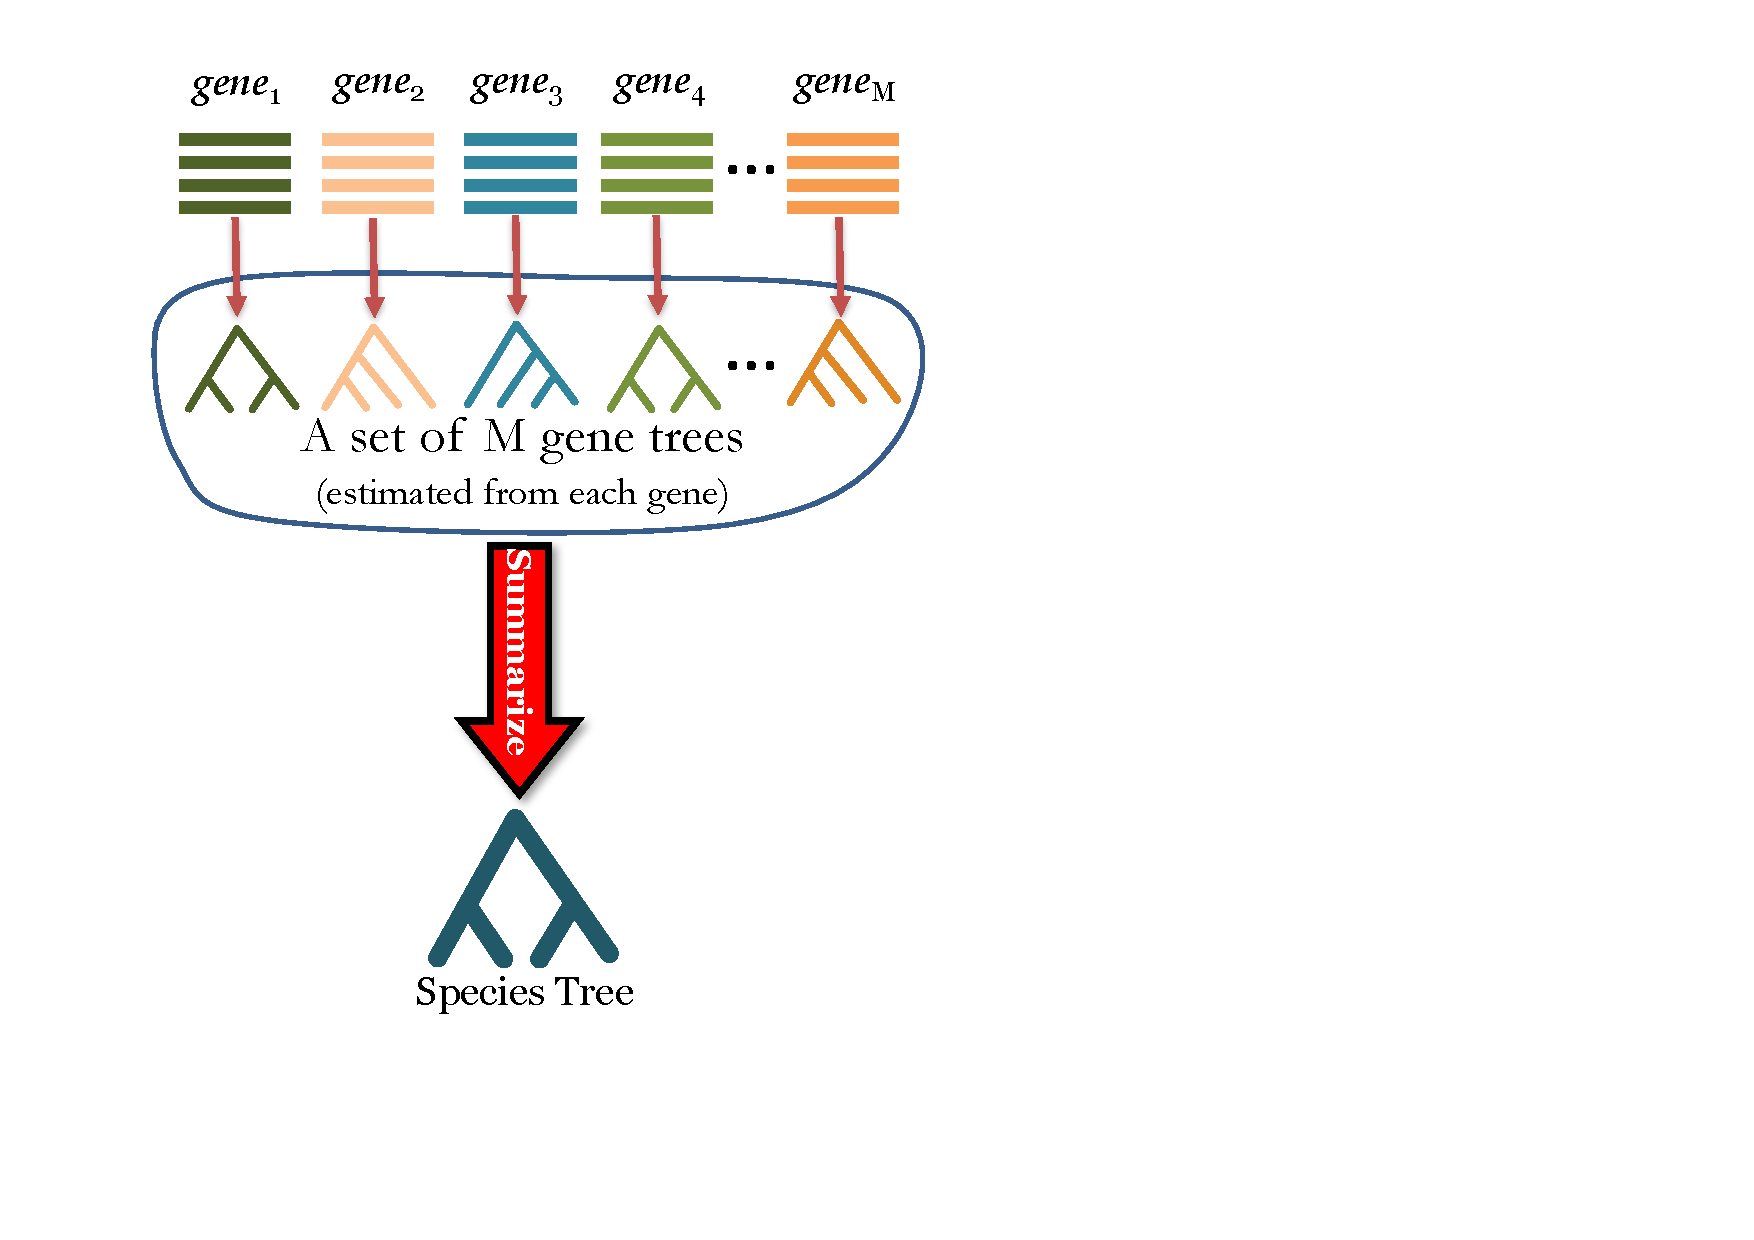
\includegraphics[width=0.4\textwidth]{Figure/summary_method}
	\caption{A visual illustration of summary method for inferring species tree.} \label{fig:summary_method}
\end{figure}

Among the newer methods, perhaps the most popular ones belong to a family called ``summary methods''~\cite{bayzid2013naive} that is illustrated in Fig.~\ref{fig:summary_method}. They take the gene trees estimated from the individual genes as input and then find a species tree that best summarizes the gene trees under various optimization criteria. 
Because incomplete lineage sorting is
expected to occur under many biologically realistic conditions (e.g., rapid radiations)~\cite{jarvis2014whole}, statistically consistent coalescent-based species tree methods have been developed and are increasingly popular. 
Examples of such methods include
MP-EST~\cite{mpest}, *BEAST~\cite{heled-drummond}, NJst~\cite{njst}, BUCKy~\cite{larget-bioinf2010}, GLASS~\cite{glass}, STEM~\cite{stem}, SNAPP~\cite{snapp}, SVDquartets~\cite{svdquartet}, STEAC~\cite{steac},
ASTRAL~\cite{mirarab2014astral}, ASTRID~\cite{vachaspati2015astrid}, and STELAR~\cite{islam2019stelar}. Each of them optimizes a particular criterion that has been shown to be statistically consistent. For instance, ASTRAL tries to find a species tree by maximizing the number of quartets in the gene trees that are consistent with it. The quartet score of the ASTRAL-estimated tree is expected to converge to the quartet score of the true tree given sufficiently large numbers of true gene trees. However, with a limited number of genes and in the presence of gene tree estimation error, existing methods may \textit{overshoot} the criterion they try to optimize, and thus may deviate from the true tree. We have observed that (please see Section~\ref{subsec:observation}), in most of the cases, quartet scores of the ASTRAL trees are more than the quartet scores of the true trees. Similarly, MP-EST, which maximizes a pseudo-likelihood measure, tends to overestimate the amount of ILS present in the gene trees~\cite{statistical-binning,bayzid2015weighted}. Moreover, the performance of various optimization criteria varies with varying model conditions~\cite{mirarab2014evaluating,chou2015comparative}.


Therefore, optimizing a particular optimization criterion, despite being statistically consistent, may not always produce highly accurate trees. This phenomenon motivates us to apply EMO techniques. 
Previously several researchers~\cite{villalobos2018memetic, santander2016performance, zambrano2016mo} successfully applied EMO approaches to infer phylogenetic trees from biological sequences. This is the first known study that aims to improve the accuracy of the species trees, estimated from a given set of gene trees, by multi-objective formulation. We reported some preliminary findings in~\cite{nayeem2020multi}.



\begin{comment}


\begin{itemize}
\item We pick three optimization scores from three different methods (ASTRAL, STELAR and MP-EST) to be simultaneously optimized by an EMO algorithm (Section~\ref{sec:problem}).  
\item We developed an NSGA-II~\cite{deb2002fast}, a popular EMO algorithm, based framework. Also, based on obtained observations, we designed a custom genetic algorithm whose final population contains a better species tree than that of the NSGA-II (Section~\ref{sec:method}). 
\item Finally based on three simulated datasets, we examine the operation of the two EMO algorithms and then compare their performance with three existing methods (Section~\ref{sec:experiment}). 
\end{itemize}
\end{comment}


 \section{Preliminaries and Problem Formulation}



\subsection{Problem Formulation}
\label{sec:problem}
Equipped with the basic concepts of phylogeny, below we formulate the task of inferring species tree as a multi-objective optimization problem (MOP).\\\\
\textbf{Input}
\begin{itemize}
	\item A set of $M$ rooted binary trees each having $N$-taxon (i.e., leaves)
\end{itemize}
\textbf{Output}
\begin{itemize}
	\item A species tree having $N$-taxon that best summarizes the input gene trees
\end{itemize}
\textbf{Objective} To estimate the species tree, we propose, for the first time, the simultaneously optimization of the following three criteria:
\begin{enumerate}[label=$F_\arabic*$)]
	\item  Maximize quartet score denoted as QT in this study
	\item  Maximize triplet score denoted as TP 
	\item  Maximize pseudo-likelihood denoted as PL    
\end{enumerate}


\begin{comment}
We are given a set of $M$ rooted binary trees as a collection gene trees each having $N$-taxon. We need to construct the species tree, a rooted binary tree with $N$-taxon, from these gene trees by simultaneously optimizing the following three objective functions:  
\begin{enumerate}[label=$F_\arabic*$)]        
\item Maximize QT 
\subitem {\scriptsize QT: number of consistent quartets (i.e., unrooted 4-taxon tree) between the species tree and the gene trees (used by ASTRAL\cite{mirarab2014astral})}
\item Maximize TP
\subitem {\scriptsize TP: number of consistent triplets (i.e., rooted 3-taxon tree) between the species tree and the gene trees (used by STELAR~\cite{islam2019stelar})}
\item Maximize PL 
\subitem {\scriptsize PL: pseudo-likelihood estimation of the species tree utilizing the underlying triplet distribution of the gene trees (used by MP-EST~\cite{mpest})}
\end{enumerate}
\end{comment}
To remain in line with the EMO literature and software frameworks, in what follows we have treated each objective as a minimization criterion. It should be noted that, although the FN rate reflects the true performance of an algorithm, it is not the fitness criterion of the EMO algorithm. Rather, the optimization continues based on the three objective values (QT, TP and PL).

Unlike classical MOPs, here our goal is not only to effectively sampling the Pareto front (PF) because of the following two issues:
\begin{enumerate}[label=$I_\arabic*$]
	\item \label{item:i1} Optimizing an objective beyond a certain limit can lead the resultant species tree to deviate (in terms of FN rate) from the true tree (please see Section~\ref{subsec:observation})
\item \label{item:i2} A solution that is badly dominated at an early generation can still potentially evolve into a highly accurate tree (in terms of FN rate) at a later generation (please see Section~\ref{subsec:issue2}; also reported in~\cite{qu2010multi})
\end{enumerate}



%
 \section{Algorithms}
\label{sec:method}
In this paper, we adapt NSGAII for species tree estimation by integrating problem-specific encoding, initialization, crossover and mutation. Moreover, we design a special purpose EMO algorithm, namely, SNOGA, by modifying NSGAII considering the issues mentioned in Section~\ref{sec:problem}. In this section, we discuss the design of our modified EMO algorithm (pseudo-code shown in Algorithm~\ref{alg:nossga}) along with its different components. In what follows, the following definition will be useful. 

\defn \label{def:domination_threshold}
{
	\small
	We call the worst value of a particular objective in the obtained PF of a certain generation as the \textbf{domination threshold} for that objective at that generation.
}

\subsection{NSGAII}
NSGAII (non-dominated sorting genetic algorithm)~\cite{deb2002fast} is a representative of Pareto non-domination based EMO algorithms and perhaps the most widely used algorithm for tackling MOPs with two or three objective functions. It follows the standard structure of a generational genetic algorithm. It starts each generation by applying the genetic operators (selection, crossover, and mutation) on the current population to generate an offspring population of the same size. Then it builds the next-generation by incorporating the best individuals from both the current and offspring populations by sorting according to a Pareto rank (i.e., non-dominated sorting ) and breaking ties (if necessary) using the concept of crowding distance. In this study, we experiment with NSGAII to analyze how a classical EMO algorithm responds to the particular issues of species tree estimation problem. 

\subsection{SNOGA}
One idea to resolve issue~\ref{item:i1}, could be to enforce a classical EMO algorithm being applied to maintain a population that contains some solutions having objective values slightly below the domination threshold (Definition~\ref{def:domination_threshold}). However, any such algorithm, in general, would continue optimizing one objective to a great extent even at the loss of some other objectives (resulting in issue~\ref{item:i1}) which may be detected through a change in sign of correlation coefficient (positive to negative)  between a pair of objectives as the generation changes. 
Therefore, we modify NSGAII to tackle issue~\ref{item:i1} in a better way than the original NSGAII in addition to resolving issue~\ref{item:i2}.  

\begin{equation}\label{eqn:nos}
SNO(x) = \sum_{i=1}^{3} \frac{F_i(x)-z_i^{min}}{z_i^{max}-z_i^{min}}
\end{equation}
Here $x$ is a candidate solution (i.e., species tree) and $z_i^{min}$ ($z_i^{max}$) is the minimum (maximum) value of $i^{th}$ objective $F_i$ observed so far during the search process.

To overcome issue~\ref{item:i2}, we avoid the concept of non-domination while selecting solutions to form the population for the next generation (line~\ref{line:next_pop1}-\ref{line:next_pop2} of Algorithm~\ref{alg:nossga}). Instead, we sort solutions (line~\ref{line:sort_nos} of Algorithm~\ref{alg:nossga}) based on the summation of normalized objective (SNO) values as defined by the $SNO()$ function in Equation~\ref{eqn:nos}. That is why, we refer to our algorithm as SNOGA, i.e, Summation of Normalized Objectives based Genetic Algorithm. We are inspired by~\cite{qu2010multi} where a similar strategy was utilized to design an EMO algorithm. Moreover, as an attempt to address issue~\ref{item:i1}, we will not allow the selection of individuals that may arise conflict (negative correlation coefficient) between any pair of objectives. We accomplish this by using the tournament selection~\cite{goldberg1991comparative} based on $SNO()$ (line~\ref{line:tournament_nos}) while forming the offspring population.
Because we expect that selection pressure based on $SNO()$ will prefer those solutions that achieve reasonably well values across all objective than those solutions which are optimized along one objective heavily at the cost of other objectives. This feature might help us to resolve or at least lessen issue~\ref{item:i1} compared to the original NSGAII algorithm (this is supported by results presented in Section~\ref{sec:experiment}). 

Additionally, we always randomly choose one from among multiple solutions having the same $SNO()$ value (line \ref{line:diversity}) to help maintain the diversity of solutions. Also, we attempt to preserve diversity by using NSGAII's crowding distance operator, albeit in a different way than NSGAII, by keeping some sparsely spaced (in the objective space) solutions having poor $SNO()$ values (line~\ref{line:crowding_s}-\ref{line:crowding_e}) in the population. In addition to doing tournament selection (as mentioned above), unlike NSGAII, we also use the random selection (line~\ref{line:random_selection}) to ensuring the participation of a few poor solutions (in terms of $SNO()$) in the offspring generating process. This increases the exploration capability of SNOGA to help escape local optima. Moreover, we expect this feature to aid in addressing issue~\ref{item:i2} as well.




\begin{algorithm}[!htbp]
\caption{SNOGA}
	\textbf{Input:} $m_g$ (max. generations), $p_s$ (population size), $c_r$ (crossover rate), $m_r$ (mutation rate), $t_s$ (tournament size)\\
	\textbf{Output:} $P$ (A list of $p_s$ candidate solutions i.e., species trees)
	\begin{algorithmic}[1]\label{alg:nossga}
		\State{$P \gets$ population\_initialization($p_s$)} \COMMENT{Sec.~\ref{subsec:init}}
		\STATE{For each solution in $ P $, evaluate the objective functions and $SNO()$ function} \COMMENT{using Eqn.\ref{eqn:nos}}
\STATE{$g \gets 0$} \COMMENT{generation counter}
		\WHILE{ $g < m_g$}
		\STATE{$Q \gets \emptyset$} \COMMENT{offspring population, an empty list that can hold $p_s$ solutions}
		\FOR{$i \leftarrow 1$ to $p_s$}    \STATE{$S_1 \gets$ tournament\_selection($P$, $t_s$)} \COMMENT{based on value of $SNO()$ function} \label{line:tournament_nos}
		\STATE{$S_2 \gets$ random\_selection($P$)} \label{line:random_selection}
		\STATE{$x \gets$ mutation(crossover($S_1, S_2, c_r$), $m_r$)}\COMMENT{Sec.~\ref{subsec:crossver}, \ref{subsec:mutation}}
		\STATE{$\!\!$Add $x$ to tail($Q$)}
\ENDFOR    
		\STATE{For each solution in $ Q $, evaluate the objective functions and $SNO()$ function }
		\STATE{$ R \gets P \cup Q$} \COMMENT{$R$ is a list holding $2p_s$ solutions}
\STATE{Sort the members of $ R $ in ascending order of $SNO()$ values} \COMMENT{ascending because all objectives are treated as minimization}\label{line:sort_nos} \label{line:nos}
		\STATE{$P \gets \emptyset$, Remove the solution from head($R$) and add it to tail($P$)} \label{line:next_pop1}
\FOR{$i \leftarrow 2$ to $p_s$}    \STATE{Remove the solution from head($R$) and store it in $x$}    \STATE{\textbf{if} $SNO$($x$) $\ne$ $SNO$(solution at tail($P$)), \textbf{then} Add $x$ to tail($P$) }    \label{line:diversity}
		
		\ENDFOR    \label{line:next_pop2}
\STATE{Sort the members of $ R $  in descending order of their crowding distance~\cite{deb2002fast} in $R$} \label{line:crowding_s}
		\STATE{Fill-up the remaining solutions for $P$ from the top of $R$}\label{line:crowding_e}
		\STATE{$g \gets g + 1$}
		\ENDWHILE
		\STATE{\textbf{return} $P$}
	\end{algorithmic}
\end{algorithm}

\subsection{Genetic Operators for NSGAII and SNOGA}
\subsubsection{Crossover}\label{subsec:crossver}
We use Prune-Delete-Graft (PDG)~\cite{villalobos2018memetic} as the crossover operator which generates one tree (i.e., offspring) from two parents. At first, it takes a random sub-tree from one of the parents. Then, it inserts the selected sub-tree in the other parent at a
randomly selected insertion point. Finally, it deletes duplicated species from the second tree and returns it as the output.

\subsubsection{Mutation} \label{subsec:mutation}
Our mutation operator applies one of the three widely used tree rearrangement strategies~\cite{felsenstein2004inferring}: (i) Nearest Neighbour
Interchange (NNI), (ii) Sub-tree Pruning and Re-grafting (SPR) and (iii) Tree Bisection and Reconnection (TBR). Each of them is selected randomly with equal probability. NNI exchanges sub-trees from an arbitrary internal branch to obtain a new tree. On the other hand, SPR picks a random sub-tree from a tree, removes it and then re-grafts it in a random position to generate a new tree. And TBR is a combination of SPR and NNI.

\subsubsection{Population Initialization}\label{subsec:init}
We generate the required number of solutions for the initial population by utilizing the given set of gene trees. To produce a single solution, we randomly pair two gene trees and apply our crossover operator on them with probability 1.0. 

\begin{comment}
\subsection{Implementation Notes}
We encode species tree using \textit{TreeTemplate} class provided by BIO++~\cite{gueguen2013bpp} which is a collection of C++ libraries for Bioinformatics. To implement NSGAII and SNOGA, we use a C++ framework for EMO, jMetalCpp~\cite{lopez2013jmetalcpp}. We reuse the implementation of PDG, NNI, SPR and TBR from~\cite{zambrano2016mo} after fixing some minor bugs therein. Furthermore, we evaluate each objective (QT/TP/PL) using a feature provided by each method (ASTRAL\footnote{\url{https://github.com/smirarab/ASTRAL/}}/STELAR\footnote{\url{https://islamazhar.github.io/STELAR/}}/MP-EST\footnote{\url{https://github.com/lliu1871/mp-est}}) to score an existing species tree. Thus for each candidate solution, we invoke the executable of a particular method to evaluate an objective. Our implementation is available at \url{https://github.com/ali-nayeem/MOP_GT2ST}.


\subsection{Objective Evaluation}
Each method (ASTRAL, STELAR or MP-EST) provides an option to score an existing species tree. We used this feature to enable to evaluate the objectives. Thus for each candidate species tree, we invoke the executable of a particular method (ASTRAL/STELAR/MP-EST) to evaluate an objective. \end{comment} 

\section{Experimental Studies}
\label{sec:experiment}
In this section, we examine the differences in the operation of NSGAII and SNOGA in terms of various aspects and evaluate their performance in comparison with three existing methods (ASTRAL, MP-EST and STELAR). ASTRAL and MP-EST are two of the most widely used and accurate summary methods~\cite{islam2019stelar}. 

\begin{table}[htbp]
	\centering
	\caption{Simulated datasets used in this study.}
	\begin{tabular}{|c|c|c|c|}
		\hline
		Dataset & \multicolumn{1}{l|}{No. of genes} & Replicates & \multicolumn{1}{l|}{Ref.} \\
		\hline
		10-taxon &   200    & R1 - R10 & \cite{bayzid2015weighted} \\
		\hline
		11-taxon &   50    & R1 - R10 & \cite{chung2011comparing} \\
		\hline
		15-taxon &   100    & R1 - R10 & \cite{statistical-binning} \\
		\hline
	\end{tabular}\label{tab:datasets}\end{table}

\begin{table*}[!htbp]
	\centering
	\small
	\caption{Parameters of our EMO algorithms.}
	\begin{tabular}{|c||c|c|} \hline
		Algo. & \multicolumn{1}{c|}{Parameter} & Value \\
		\hline
		\multirow{6}{*}{All} & Max. generations & 99 \\	
		\cline{2-3}          & Population size & 100 \\ \cline{2-3} & Max. fitness evaluation & 10000 \\	
		\cline{2-3}          &  Mutation & Randomly from \{NNI, SPR, TBR\}~\ref{subsec:mutation} \\
		\cline{2-3}          & Mutation rate & 1.0 \\
		\cline{2-3}          & Crossover  & PDG~\ref{subsec:crossver} \\
		\cline{2-3}          & Crossover rate & 0.3 \\ \cline{2-3}          & No. of repeated runs & 15 \\
		\hline \hline
		\multirow{1}{*}{NSGAII} & Selection & Binary tournament based on Pareto domination \\ \hline \hline
		\multirow{2}{*}{SNOGA} & Selection & Random,  tournament based on Eqn.\ref{eqn:nos} \\ \cline{2-3}          & Tournament size & 10 \\ \hline
	\end{tabular}\label{tab:parameters}\end{table*}\subsection{Experimental Setting}
\subsubsection{Implementation notes}
The implementation of our EMO algorithms are available at \url{https://github.com/ali-nayeem/MOP_GT2ST}. We encode species tree using \textit{TreeTemplate} class provided by BIO++~\cite{gueguen2013bpp} which is a collection of C++ libraries for Bioinformatics. To implement NSGAII and SNOGA, we use a C++ framework for EMO, jMetalCpp~\cite{lopez2013jmetalcpp}. We reuse the implementation of PDG, NNI, SPR and TBR from~\cite{zambrano2016mo} after fixing some minor bugs therein. Furthermore, currently we evaluate each objective (QT/TP/PL) using a feature provided by each method (ASTRAL\footnote{\url{https://github.com/smirarab/ASTRAL/}}/STELAR\footnote{\url{https://islamazhar.github.io/STELAR/}}/MP-EST\footnote{\url{https://github.com/lliu1871/mp-est}}) to score an existing species tree. Thus for each candidate solution, we invoke the executable of a particular method to evaluate an objective. Due to this external dependency, the runtime of our EMO algorithms increased a lot. We ran experiments using a machine with Intel \textsuperscript{\textregistered} Core\textsuperscript{TM} i7-3770 @ 3.40GHz and 8 GB of RAM under Ubuntu 16.04.


\subsubsection{Datasets}
We used three simulated datasets listed in Table~\ref{tab:datasets}. For each dataset, we include 10 replicates (R1 to R10). In this
context, a replicate means a randomly generated instance of the simulated dataset based on the
 given model condition. These datasets are relatively smaller which helps us to cope with our large runtime caused by the use of external tools for fitness evaluations.
We used False Negative (FN) rate~\cite{bayzid2013naive} to measure the accuracy of the estimated species tree. FN rate expresses the fraction of edges present in the true species tree (Provided with the dataset) but missing in the estimated tree. Thus the calculated FN rate of the solutions finally returned by an algorithm reflects the actual performance of that algorithm concerning the application (i.e., species tree estimation).

\subsubsection{Parameter setting}
The parameters of our EMO algorithms are listed in Table~\ref{tab:parameters}. We fix these parameters empirically. In our context, mutation is more useful than crossover as the later can produce an offspring that is very different from the parent. It should be noted that, we used maximum generations as 99 and repeated runs as 15 to cope with the large runtime resulting from the dependency on external tools. 
For comparison, we collected the trees estimated by ASTRAL, STELAR and MP-EST from~\cite{islam2019stelar}. They ran the exact version of ASTRAL and STELAR, which are guaranteed to return the globally optimal tree. And for MP-EST, they ran with 10 random starting points and selected the species tree with the best PL value.   




\begin{figure*}[!htbp]
\centering    
		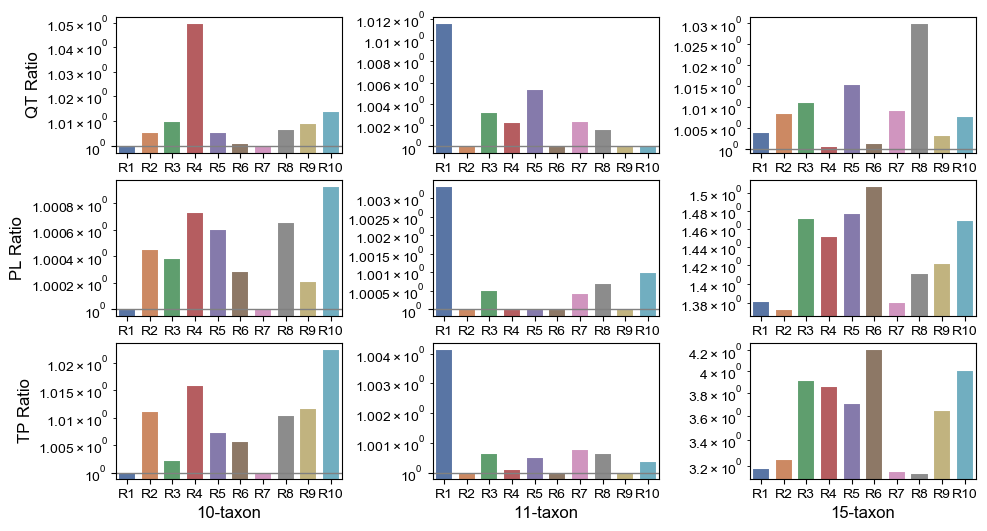
\includegraphics[width=1\textwidth]{Figure/tool_ratio}
\caption{The issue of overshooting the optimization criterion beyond the true tree by existing methods. Each row shows the ratio of scores (QT/PL/TP), optimized by a particular method (ASTRAL/MP-EST/STELAR), of the true tree to that of the estimated tree by the same method.} \label{fig:tool_ratio}
\end{figure*}

\subsection{Overshooting of Optimization Criterion}
\label{subsec:observation}
At first, we present an important observation that essentially motivated us to tackle the problem of species tree estimation as a MOP. As we mentioned in Section~\ref{sec:intro}, existing methods may overshoot the criterion they try to optimize, and thus may deviate from the true tree. In Fig.~\ref{fig:tool_ratio}, we summarize our observations for three methods (ASTRAL, MP-EST and STELAR) on 10 replicates of our selected datasets. Here, the top row shows the ratio of quartet-scores (QT) of the true trees to quartet-scores (QT) of the ASTRAL-estimated trees. Likewise, the middle row shows the pseudo-likelihood (PL) ratio of the true trees and MP-EST estimated trees and the bottom row does the same with the triplet (TP) ratio of STELAR. As we treat each objective as a minimization task, ideally these ratios should be 1 (marked as a gray horizontal line in each plot). However, we find that in most of the cases the ratio is greater than 1 implying that the results have been over-optimized. 


\subsection{NSGAII vs. SNOGA}
Now we closely inspect the behavioral difference between NSGAII and SNOGA to find out how SNOGA addresses the two issues (mentioned in Section~\ref{sec:problem}) in comparison with NSGAII. To ensure a level playing field, we executed both algorithms with the same configuration as reported in Table~\ref{tab:parameters}. 

\begin{figure*}[!htbp]
\centering
\begin{subfigure}[b]{0.33\textwidth}
			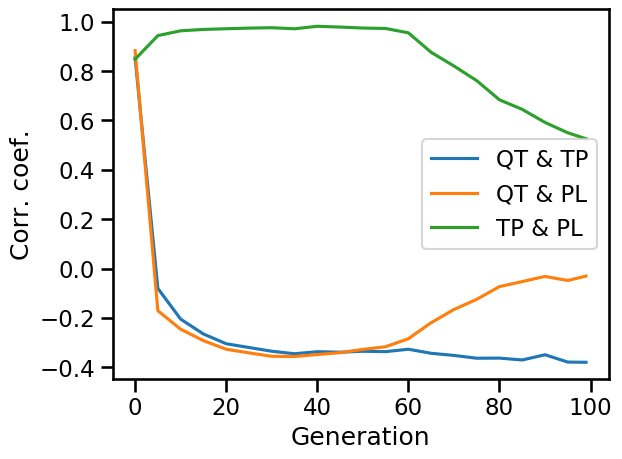
\includegraphics[width=\textwidth]{Figure/10-taxon_NSGAII_corr_plot}
			\caption{NSGAII: 10-taxon}
\end{subfigure}\begin{subfigure}[b]{0.33\textwidth}
			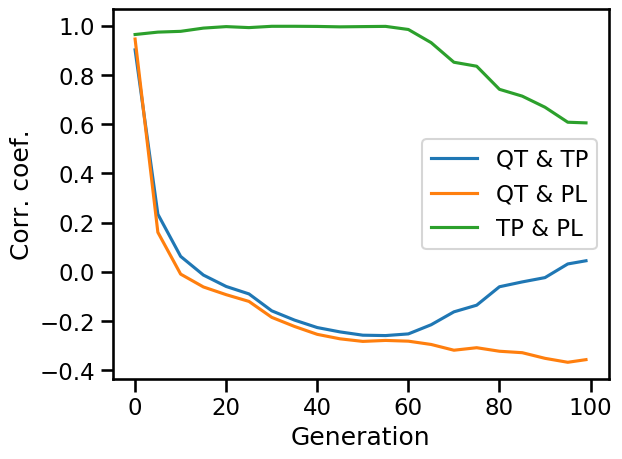
\includegraphics[width=\textwidth]{Figure/11-taxon_NSGAII_corr_plot}
			\caption{NSGAII: 11-taxon}
\end{subfigure}\begin{subfigure}[b]{0.33\textwidth}
			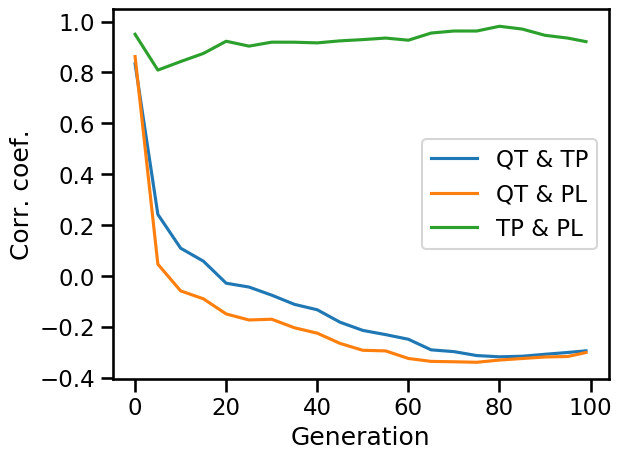
\includegraphics[width=\textwidth]{Figure/15-taxon_NSGAII_corr_plot}
			\caption{NSGAII: 15-taxon}
\end{subfigure}    
		\begin{subfigure}[b]{0.33\textwidth}
			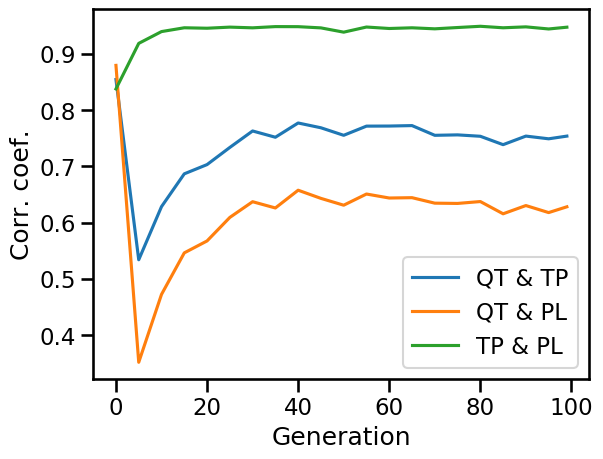
\includegraphics[width=\textwidth]{Figure/10-taxon_NOSSGA_corr_plot}
			\caption{SNOGA: 10-taxon}
\end{subfigure}\begin{subfigure}[b]{0.33\textwidth}
			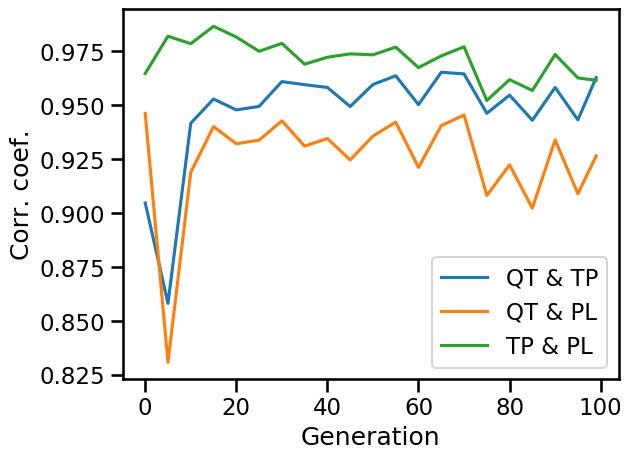
\includegraphics[width=\textwidth]{Figure/11-taxon_NOSSGA_corr_plot}
			\caption{SNOGA: 11-taxon}
\end{subfigure}\begin{subfigure}[b]{0.33\textwidth}
			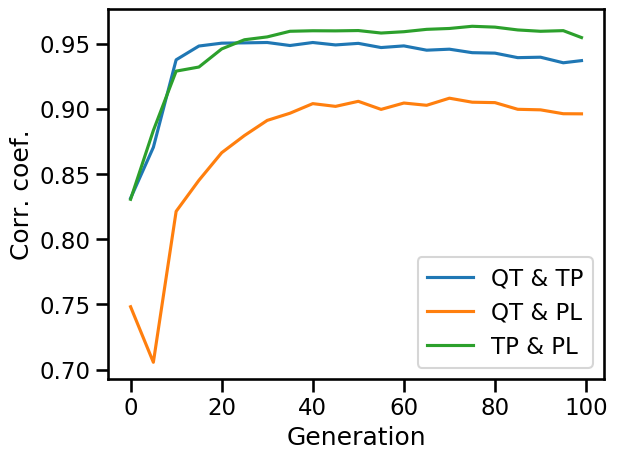
\includegraphics[width=\textwidth]{Figure/15-taxon_NOSSGA_corr_plot}
			\caption{SNOGA: 15-taxon}
\end{subfigure}
		\caption{Correlations between each pair of objectives against generations for NSGAII and SNOGA on three datasets.}
		\label{fig:gen_wise_correlation}
\end{figure*}

\subsubsection{Correlation between two objectives} We plot the correlation coefficients between each pair of objectives against different generations for NSGAII and SNOGA on three datasets in Fig.~\ref{fig:gen_wise_correlation}. Here the horizontal axis represents the generations and the vertical axis represents the correlation coefficients averaged over 15 runs and 10 replicates. We see that, contrary to NSGAII, SNOGA does not exhibit any negative correlation coefficient between any pair of objectives. These results suggest that SNOGA is able to prevent the optimization of one objective to a great extent even at the loss of some other objectives, thereby alleviating issue~\ref{item:i1} (mentioned in Section~\ref{sec:problem}) to some extent.

\begin{figure*}[!htbp]
	\centering
\begin{subfigure}[b]{0.33\textwidth}
			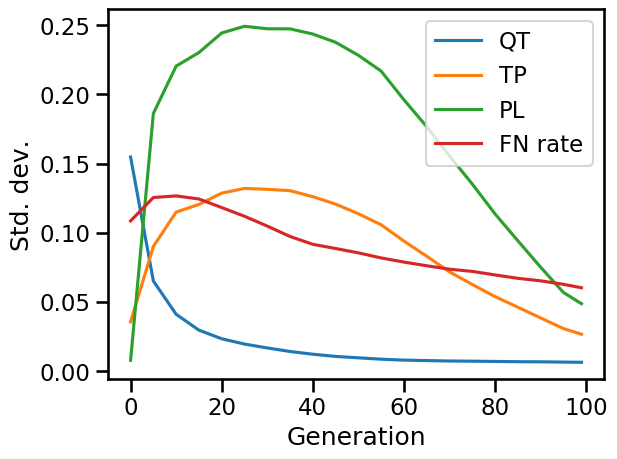
\includegraphics[width=\textwidth]{Figure/10-taxon_NSGAII_std_dev}
			\caption{NSGAII: 10-taxon}
\end{subfigure}\begin{subfigure}[b]{0.33\textwidth}
			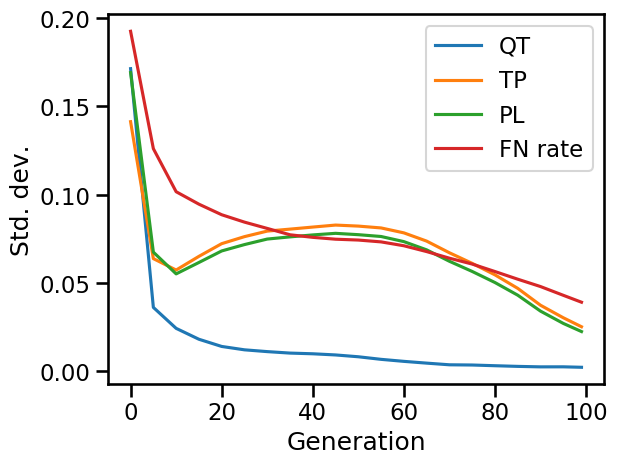
\includegraphics[width=\textwidth]{Figure/11-taxon_NSGAII_std_dev}
			\caption{NSGAII: 11-taxon}
\end{subfigure}\begin{subfigure}[b]{0.33\textwidth}
			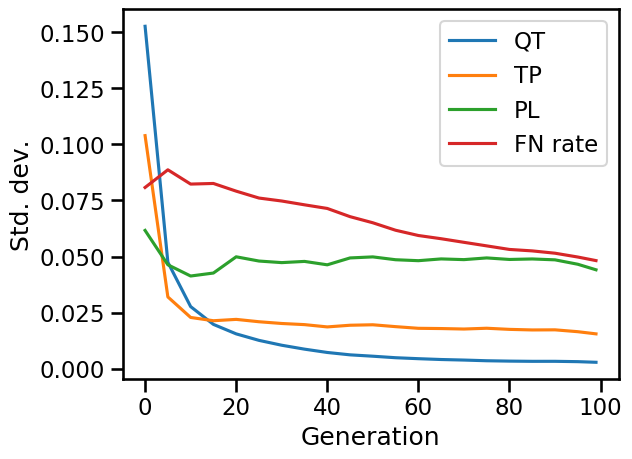
\includegraphics[width=\textwidth]{Figure/15-taxon_NSGAII_std_dev}
			\caption{NSGAII: 15-taxon}
\end{subfigure}
		\begin{subfigure}[b]{0.33\textwidth}
			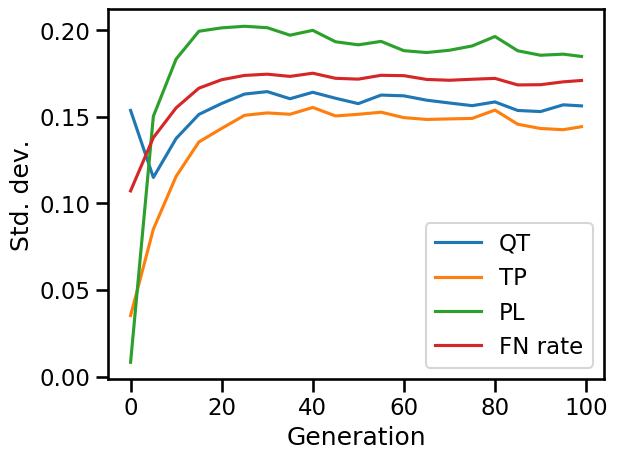
\includegraphics[width=\textwidth]{Figure/10-taxon_NOSSGA_std_dev}
			\caption{SNOGA: 10-taxon}
\end{subfigure}\begin{subfigure}[b]{0.33\textwidth}
			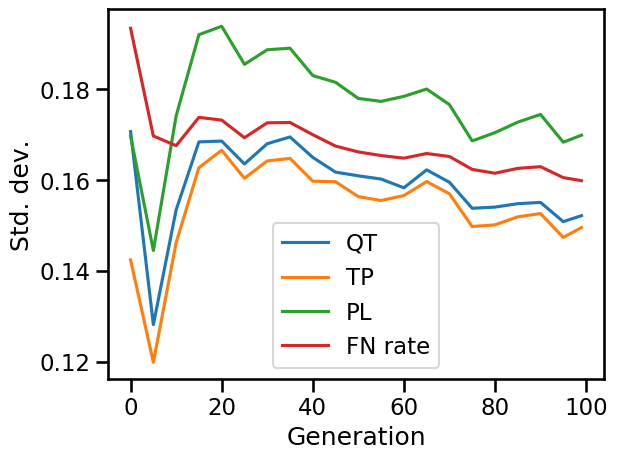
\includegraphics[width=\textwidth]{Figure/11-taxon_NOSSGA_std_dev}
			\caption{SNOGA: 11-taxon}
\end{subfigure}\begin{subfigure}[b]{0.33\textwidth}
			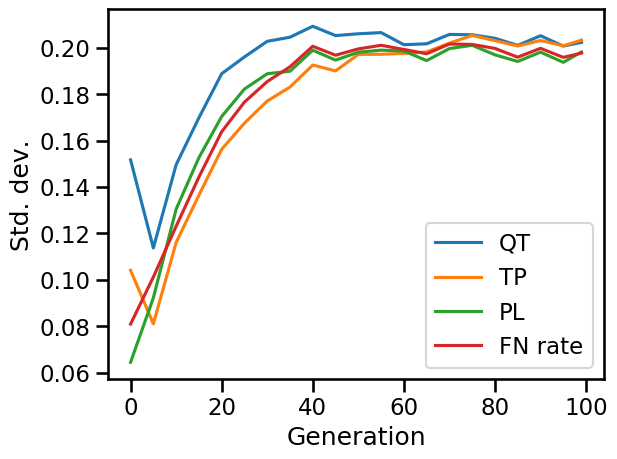
\includegraphics[width=\textwidth]{Figure/15-taxon_NOSSGA_std_dev}
			\caption{SNOGA: 15-taxon}
\end{subfigure}
		\caption{Variation of standard deviation of three objectives and FN rates in the population with generations for NSGAII and SNOGA on three datasets.}
		\label{fig:gen_wise_std_dev}
\end{figure*}

\subsubsection{Diversity of objectives and FN rate}\label{subsubsec:diversity} Fig.~\ref{fig:gen_wise_std_dev} shows the variation of the standard deviation of three objective values (normalized using global maximum and minimum) of the population members and their respective FN rates in the population with generations for NSGAII and SNOGA on three datasets. Along the vertical axis, we plotted the standard deviation values averaged over 15 runs and 10 replicates. We find that SNOGA can maintain diversity throughout the generations presumably owing to the steps taken to mitigate issue~\ref{item:i2} which we discussed in Section~\ref{sec:method}. On the other hand, NSGAII loses diversity at an early stage.


\begin{figure*}[!h]
	\centering
\begin{subfigure}[b]{0.33\textwidth}
			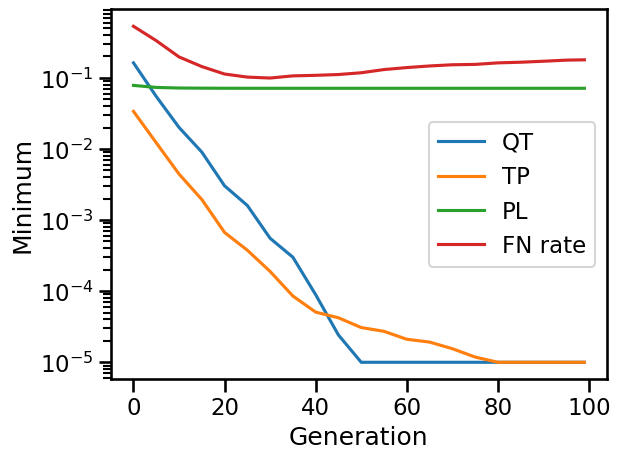
\includegraphics[width=\textwidth]{Figure/10-taxon_NSGAII_minimum}
			\caption{NSGAII: 10-taxon}
\end{subfigure}\begin{subfigure}[b]{0.33\textwidth}
			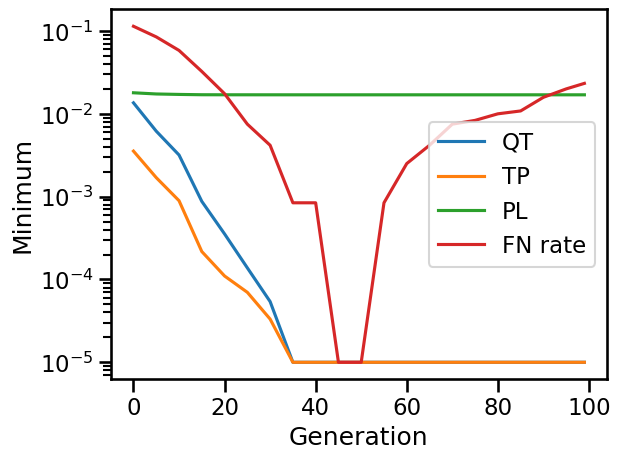
\includegraphics[width=\textwidth]{Figure/11-taxon_NSGAII_minimum}
			\caption{NSGAII: 11-taxon}
\end{subfigure}\begin{subfigure}[b]{0.33\textwidth}
			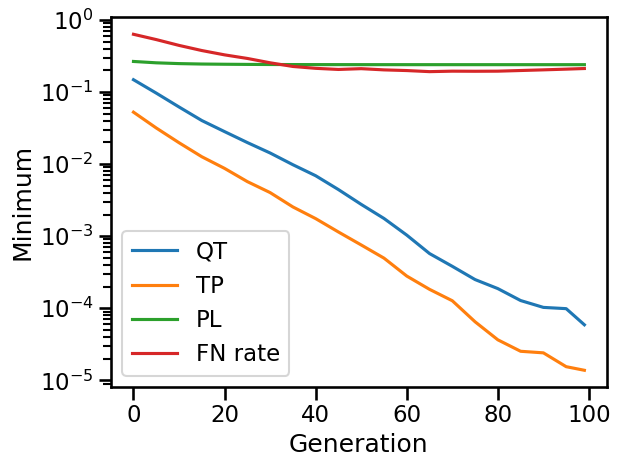
\includegraphics[width=\textwidth]{Figure/15-taxon_NSGAII_minimum}
			\caption{NSGAII: 15-taxon}
\end{subfigure}
		\begin{subfigure}[b]{0.33\textwidth}
			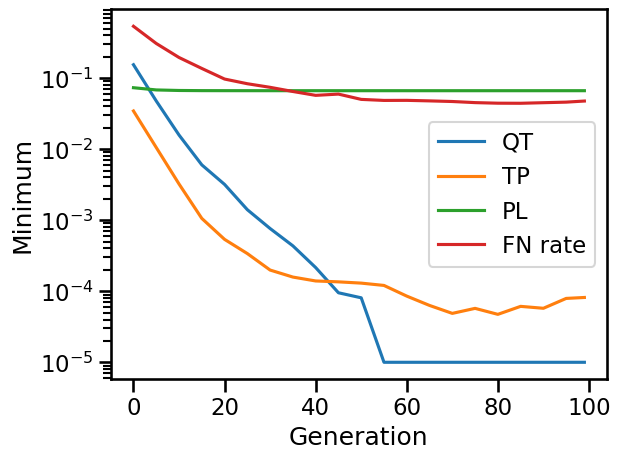
\includegraphics[width=\textwidth]{Figure/10-taxon_NOSSGA_minimum}
			\caption{SNOGA: 10-taxon}
\end{subfigure}\begin{subfigure}[b]{0.33\textwidth}
			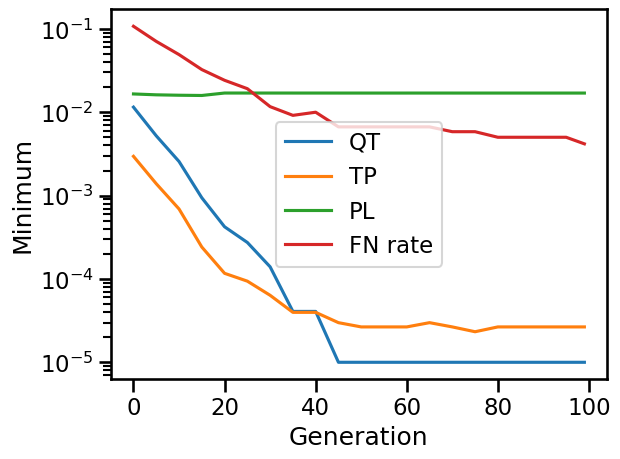
\includegraphics[width=\textwidth]{Figure/11-taxon_NOSSGA_minimum}
			\caption{SNOGA: 11-taxon}
\end{subfigure}\begin{subfigure}[b]{0.33\textwidth}
			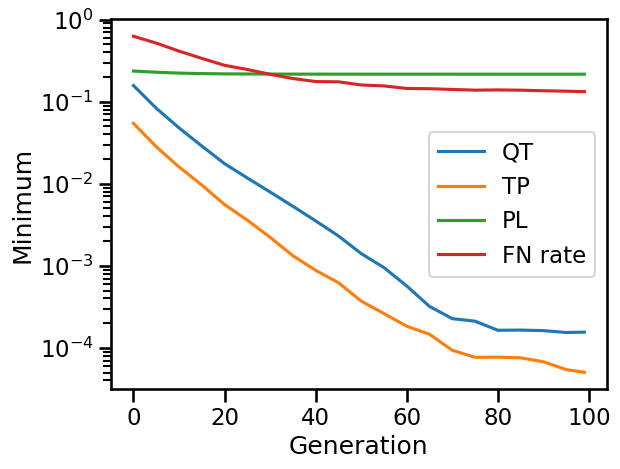
\includegraphics[width=\textwidth]{Figure/15-taxon_NOSSGA_minimum}
			\caption{SNOGA: 15-taxon}
\end{subfigure}
		\caption{Variation of minimum of three objectives (individually) and FN rates in the population with generations for NSGAII and SNOGA on three datasets.	}
		\label{fig:gen_wise_min}
\end{figure*}

\subsubsection{Improvement of FN rate vs. individual objectives} Now we observe how the best (minimum) value of three objectives (individually) and FN rate (lower is better) in the population behave across generations for NSGAII and SNOGA as depicted in Fig.~\ref{fig:gen_wise_min}. The plotted values are averaged over 15 runs and 10 replicates. We mentioned earlier that FN rate reflects the true performance of an algorithm. However, the FN rate is not the fitness criterion of the optimization process. Rather, the optimization continues based on the three objective values (QT, TP and PL).
We see that, NSGAII allows one or more objectives to improve as much as possible which may cause the resultant species tree to deviate from the true tree (issue~\ref{item:i1}). As a result, the best FN rate of NSGAII starts to degrade after a particular generation despite continuous improvement of some objectives. For example, in Fig.~\ref{fig:gen_wise_min}(a), NSGAII achieves the best FN rate at around $ 30^{th} $ generation. Afterwards, the FN rate starts to degrade. However, QT and TP continue to improve until $ 50^{th} $ and $ 80^{th} $ generation respectively.
On the other hand, to avoid such deviation, SNOGA in effect, restricts the improvement of one or more objectives after certain number of generation. So its FN rate continues to improve. From these results, we can see that SNOGA is more effective than NSGAII in dealing with issue~\ref{item:i1}.


\subsubsection{Comparison based on hypervolume} We mentioned in Section~\ref{sec:problem} that the problem that we deal with in this paper is different from the traditional MOPs. Importantly, the definition of convergence for MOPs is not the same as the convergence within the context of this problem. To explore this issue, we compare NSGAII and SNOGA in terms of hypervolume (HV)~\cite{zitzler1999multiobjective} which is probably the most popular performance measure used for MOPs. HV captures both convergence and diversity of the PF, sampled by an EMO algorithm, in a single real-value. To calculate HV, we normalized each objective value using global maximum and minimum and then used $(1.1, 1.1, 1.1)^T$ as the reference point. For MOPs with all minimization objectives, a higher value of HV is desirable. In Fig.~\ref{fig:gen_wise_hv}, we plot the HV values for NSGAII and SNOGA which are averaged over 15 runs and 10 replicates. From these results, it is difficult to differentiate between these two algorithms. Both HV values get saturated at an early generation. Even, according to HV, SNOGA seems better than NSGAII more strikingly so for the larger dataset. The reason for worse value of NSGAII concerning HV could be attributed to the loss of diversity, as exhibited by it, at an early stage. 

\begin{figure*}[!htbp]
	\centering
\begin{subfigure}[b]{0.33\textwidth}
			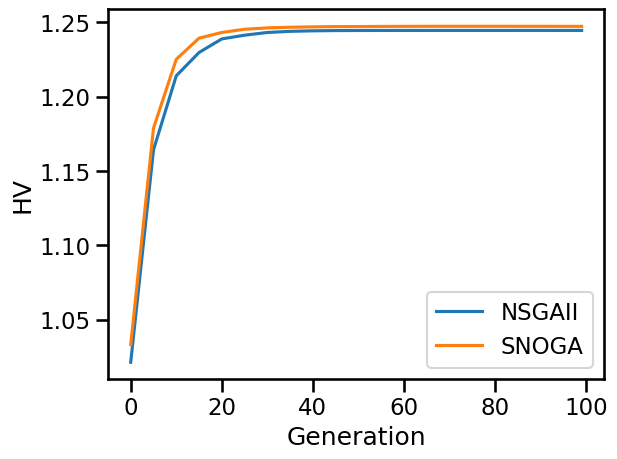
\includegraphics[width=\textwidth]{Figure/10-taxon_hv}
			\caption{10-taxon}
\end{subfigure}\begin{subfigure}[b]{0.33\textwidth}
			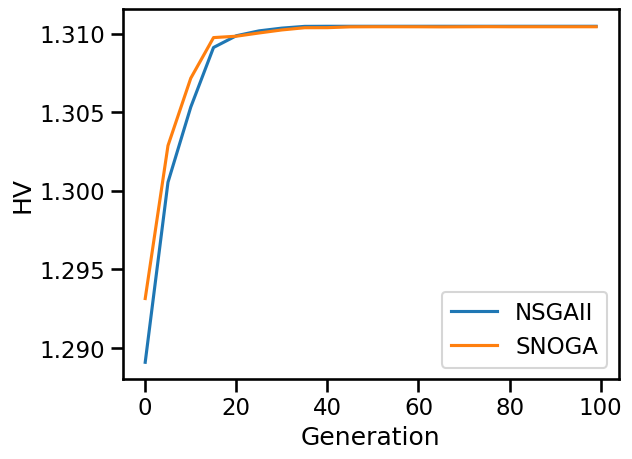
\includegraphics[width=\textwidth]{Figure/11-taxon_hv}
			\caption{11-taxon}
\end{subfigure}\begin{subfigure}[b]{0.33\textwidth}
			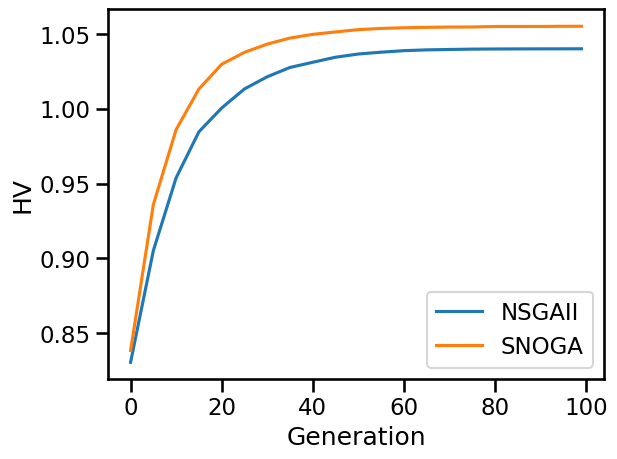
\includegraphics[width=\textwidth]{Figure/15-taxon_hv}
			\caption{15-taxon}
\end{subfigure}
		\caption{Variation of HV with generations for NSGAII and SNOGA on three datasets.}
		\label{fig:gen_wise_hv}
\end{figure*}

\begin{figure*} [!htbp]
	\centering
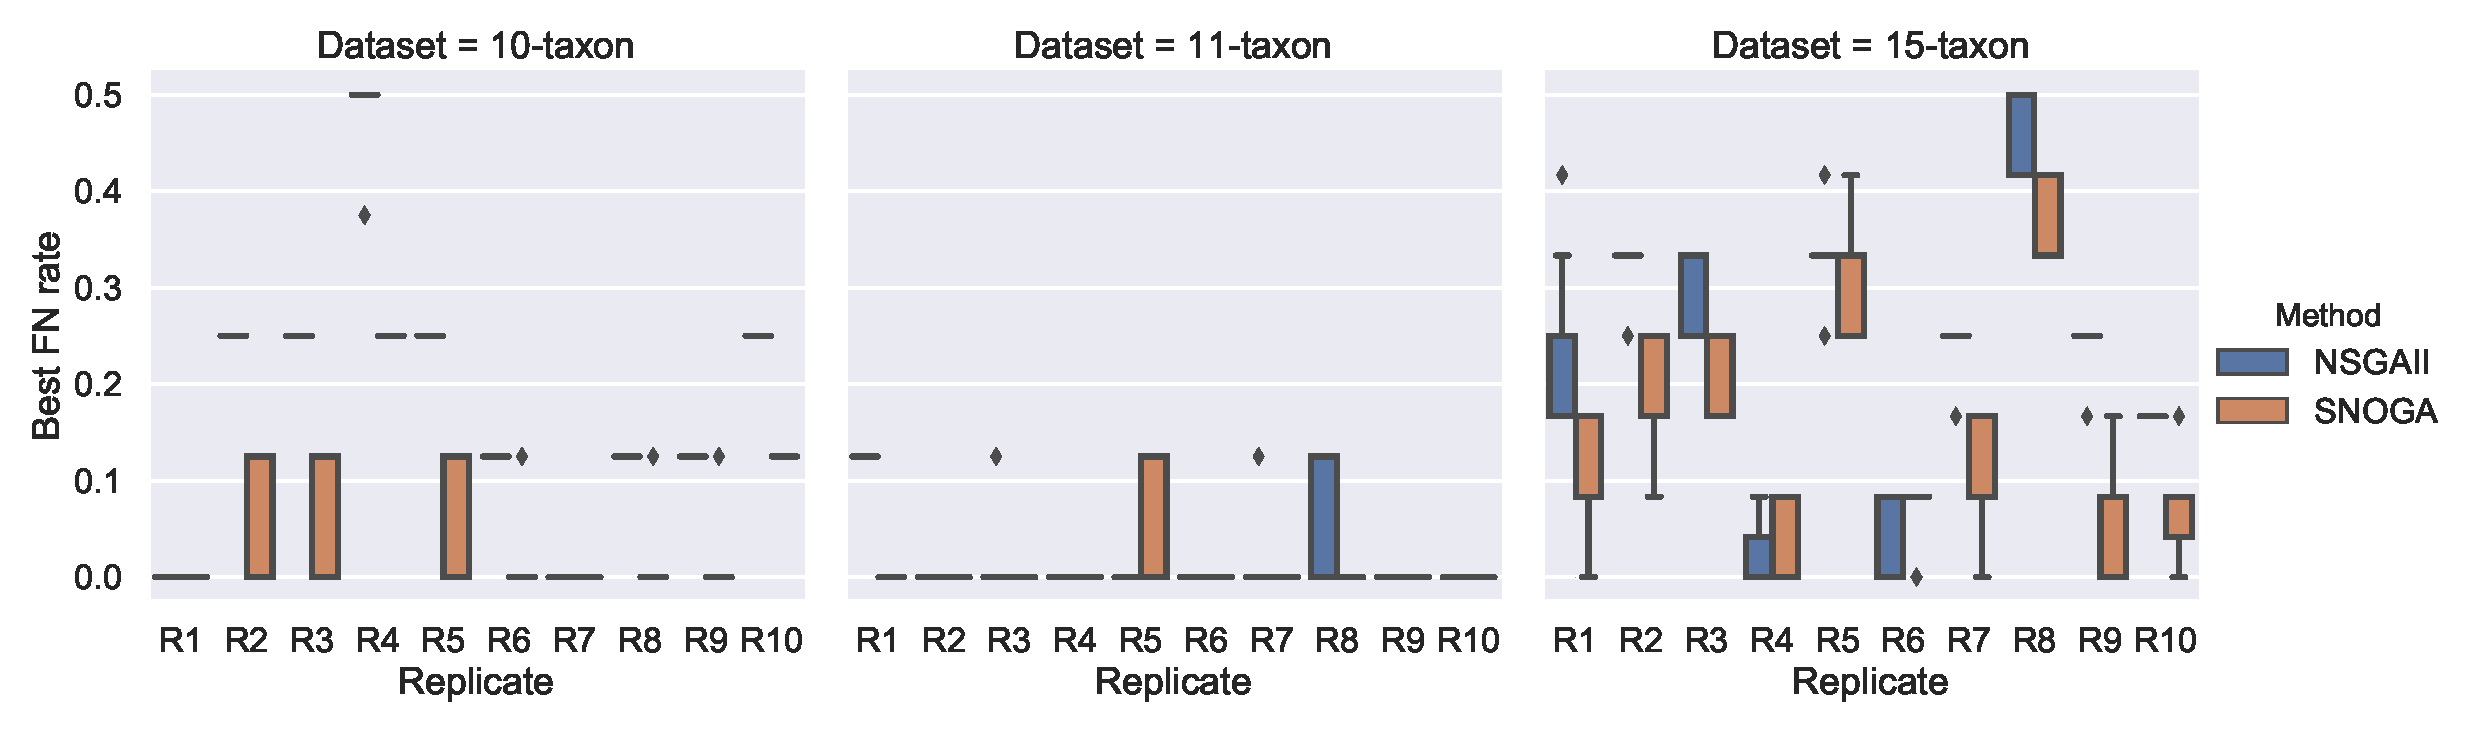
\includegraphics[width=1\textwidth]{Figure/emo_boxplot}
\caption{Accuracy (i.e., FN rate) of the best estimated species trees extracted from the final population of NSGAII and SNOGA on each dataset having 10 replicate.} \label{fig:emo_compare}	
\end{figure*}


\npdecimalsign{.}
\nprounddigits{4}
\begin{table}[htbp]
	\scriptsize
	\centering
	\caption{Summary of FN rates achieved by NSGAII and SNOGA on 10 replicates of three datasets over 15 independent runs.}
	\begin{tabular}{|c|l|n{1}{1}|n{1}{1}||n{1}{1}|n{1}{1}|}
		\hline
		\multirow{2}{*}{Dataset} & \multicolumn{1}{c|}{\multirow{2}{*}{Rep.}} & \multicolumn{2}{c||}{NSGAII} & \multicolumn{2}{c|}{SNOGA} \\
		\cline{3-6}          &       & \multicolumn{1}{l|}{Average} & \multicolumn{1}{l||}{Std. Dev.} & \multicolumn{1}{l|}{Average} & \multicolumn{1}{l|}{Std. Dev.} \\
		\hline
		\multirow{10}{*}{10-taxon} & R1    & 0     & 0     & 0     & 0 \\
		\cline{2-6}          & R2    & 0.25  & 0     & 0.0583333 & 0.062360956 \\
		\cline{2-6}          & R3    & 0.25  & 0     & 0.0666667 & 0.062360956 \\
		\cline{2-6}          & R4    & 0.4916667 & 0.031180478 & 0.25  & 0 \\
		\cline{2-6}          & R5    & 0.25  & 0     & 0.05  & 0.061237244 \\
		\cline{2-6}          & R6    & 0.125 & 0     & 0.0083333 & 0.031180478 \\
		\cline{2-6}          & R7    & 0     & 0     & 0     & 0 \\
		\cline{2-6}          & R8    & 0.125 & 0     & 0.0166667 & 0.042491829 \\
		\cline{2-6}          & R9    & 0.125 & 0     & 0.0083333 & 0.031180478 \\
		\cline{2-6}          & R10   & 0.25  & 0     & 0.125 & 0 \\
		\hline \hline
		\multirow{10}{*}{11-taxon} & R1    & 0.125 & 0     & 0     & 0 \\
		\cline{2-6}          & R2    & 0     & 0     & 0     & 0 \\
		\cline{2-6}          & R3    & 0.0166667 & 0.042491829 & 0     & 0 \\
		\cline{2-6}          & R4    & 0     & 0     & 0     & 0 \\
		\cline{2-6}          & R5    & 0     & 0     & 0.0416667 & 0.058925565 \\
		\cline{2-6}          & R6    & 0     & 0     & 0     & 0 \\
		\cline{2-6}          & R7    & 0.025 & 0.05  & 0     & 0 \\
		\cline{2-6}          & R8    & 0.0666667 & 0.062360956 & 0     & 0 \\
		\cline{2-6}          & R9    & 0     & 0     & 0     & 0 \\
		\cline{2-6}          & R10   & 0     & 0     & 0     & 0 \\
		\hline \hline
		\multirow{10}{*}{15-taxon} & R1    & 0.2166667 & 0.073282811 & 0.1111111 & 0.0496904 \\
		\cline{2-6}          & R2    & 0.3166667 & 0.033333333 & 0.1944444 & 0.049690399 \\
		\cline{2-6}          & R3    & 0.3055556 & 0.03928371 & 0.2166667 & 0.040824829 \\
		\cline{2-6}          & R4    & 0.0222222 & 0.036851387 & 0.0555556 & 0.03928371 \\
		\cline{2-6}          & R5    & 0.3333333 & 0.030429031 & 0.3111111 & 0.056655772 \\
		\cline{2-6}          & R6    & 0.0444444 & 0.041573971 & 0.0666667 & 0.033333333 \\
		\cline{2-6}          & R7    & 0.2444444 & 0.020786985 & 0.1333333 & 0.050917508 \\
		\cline{2-6}          & R8    & 0.4611111 & 0.041573971 & 0.3777778 & 0.041573971 \\
		\cline{2-6}          & R9    & 0.2444444 & 0.020786985 & 0.0555556 & 0.0496904 \\
		\cline{2-6}          & R10   & 0.1666667 & 0     & 0.0666667 & 0.045133547 \\
		\hline
	\end{tabular}\label{tab:emo}\end{table}

\subsubsection{Comparison based on tree accuracy}\label{subsec:issue2} Next, we compare NSGAII and SNOGA in terms of the tree accuracy for 10 replicates of each dataset. We measure tree accuracy in terms of the FN rate. A lower value of the FN rate corresponds to higher accuracy. We visualize the FN rates of the best trees obtained from the final population of 15 independent runs using boxplots in Fig.~\ref{fig:emo_compare}. Also, we summarize these results in Table~\ref{tab:emo}. We observe that SNOGA can offer much better trees than NSGAII in most of the 30 instances, whereas NSGAII outperforms SNOGA only on three cases (11-taxon: R5; 15-taxon: R4, R6). In some situations, two algorithms perform equally. We performed a standard paired $ t $-test based on the average FN rates achieved by NSGAII and SNOGA  (reported in Table~\ref{tab:emo}; this data satisfies the condition of normality and homoscedasticity~\cite{sheskin2003handbook}) and found significant difference ($t$-statistic: 5.20080, $p$-value: 0.00001) between them.

\begin{figure*}[!h]
	\centering
\begin{subfigure}[b]{0.33\textwidth}
		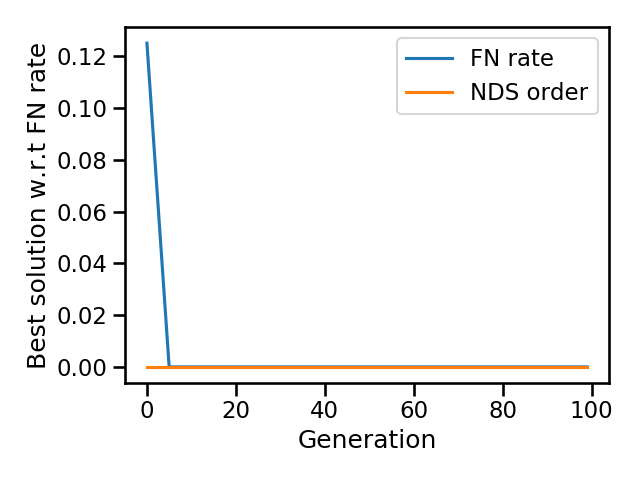
\includegraphics[width=\textwidth]{Figure/11-taxon_R5_runx_nds_order}
		\caption{11-taxon: R5}
\end{subfigure}\begin{subfigure}[b]{0.33\textwidth}
		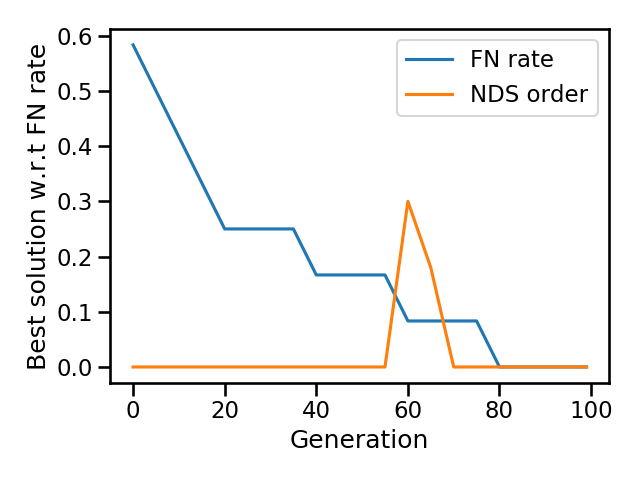
\includegraphics[width=\textwidth]{Figure/15-taxon_R4_run2_nds_order}
		\caption{15-taxon: R4}
\end{subfigure}\begin{subfigure}[b]{0.33\textwidth}
		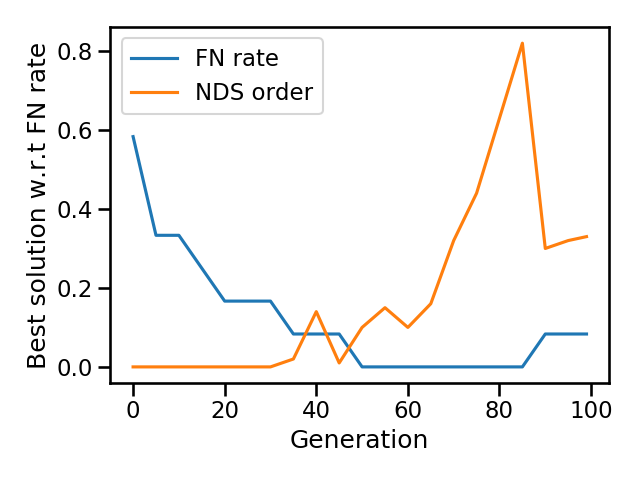
\includegraphics[width=\textwidth]{Figure/15-taxon_R6_runx_nds_order}
		\caption{15-taxon: R6}
\end{subfigure}
	\begin{subfigure}[b]{0.33\textwidth}
		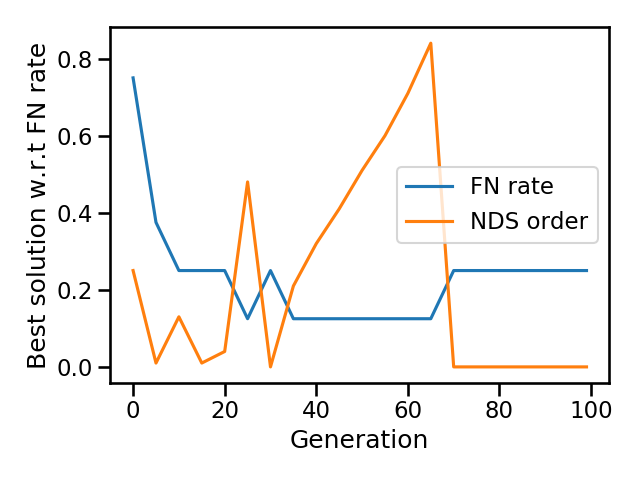
\includegraphics[width=\textwidth]{Figure/10-taxon_R5_run2_nds_order}
		\caption{10-taxon: R5}
\end{subfigure}\begin{subfigure}[b]{0.33\textwidth}
		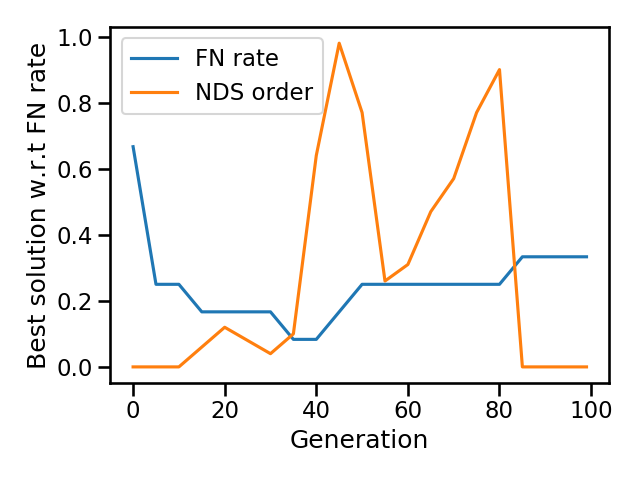
\includegraphics[width=\textwidth]{Figure/15-taxon_R3_run1_nds_order}
		\caption{15-taxon: R3}
\end{subfigure}\begin{subfigure}[b]{0.33\textwidth}
		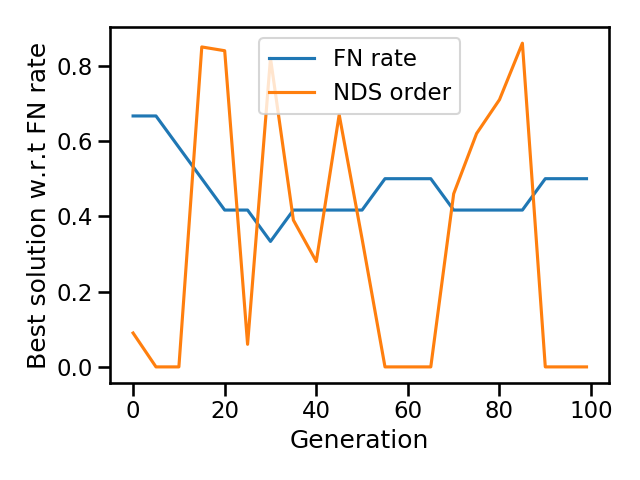
\includegraphics[width=\textwidth]{Figure/15-taxon_R8_run1_nds_order}
		\caption{15-taxon: R8}
\end{subfigure}
	\caption{State of the best solution (having the lowest FN rate) in the population with generations in terms of NDS order for NSGAII on six instances. }
	\label{fig:nsgaii_issue2}
\end{figure*}

Now we investigate why SNOGA is outperformed by NSGAII in three instances (11-taxon: R5; 15-taxon: R4, R6). To accomplish this, we examine the best solution according to the FN rate in the population across each generation in terms of its order in the population determined by the non-dominated sorting. We call this order as NDS order which is a real value between 0 and 1. For example, if the NDS order of the best solution (i.e., lowest FN rate) is 0, it means that solution is dominated by none in the current population. On the other hand, NDS order 0.8 means that the best solution is dominated by 80\% members of the current population. A larger value of NDS order indicates the higher likelihood of excluding that solution from the next generation which causes degradation in the FN rate. In other words, the NDS order of the best solution across different generations of NSGAII can offer an exhibition of issue~\ref{item:i2}. In Fig.~\ref{fig:nsgaii_issue2}, the top row exhibits the three cases where NSGAII outperformed SNOGA and the bottom row represents three arbitrary examples of other cases. We find that, in the top row, somehow the extent of issue~\ref{item:i2} is limited which is a possible reason for the superior performance of NSGAII in those cases. However, the bottom row reveals the usual scenario which is troublesome for any Pareto domination based algorithm like NSGAII. 

\subsection{2-objectives vs. 3-objectives}
Here we compare the performance of our 3-objectives formulation (i.e., {QT, TP, PL}) with that of the 2-objective formulations (i.e., {QT, TP}, {TP, PL} and {QT, PL}) in terms of FN rates averaged over 10 replicates. Fig.~\ref{fig:obj_wise_perf} shows the average FN rates with standard error bars for each dataset. We see that, for 10-taxon and 11-taxon datasets {QT, TP} and {QT, PL} can offer slightly better results than {QT, TP, PL}. This also shows QT to be a better estimator of the true species tree than the other two objectives. However, in the case of larger search space (i.e., 15-taxon dataset) {QT, TP, PL} starts to outperform others. This indicates that for larger datasets, including more objectives in the formulation increases the chance of achieving higher accuracy.

\begin{figure*}[!htbp]
	\centering
\begin{subfigure}[b]{0.33\textwidth}
		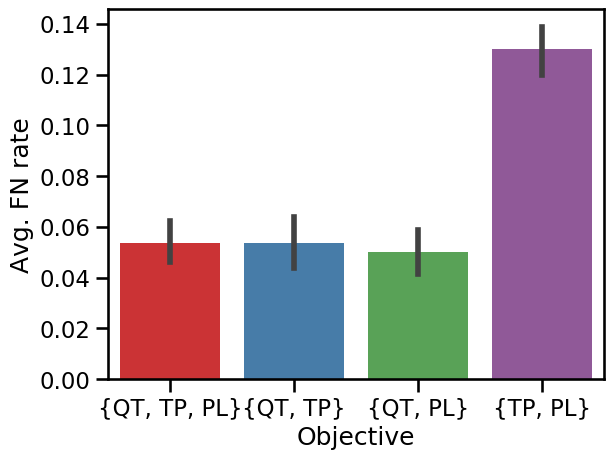
\includegraphics[width=\textwidth]{Figure/10-taxon_obj_wise_perf}
		\caption{10-taxon}
\end{subfigure}\begin{subfigure}[b]{0.33\textwidth}
		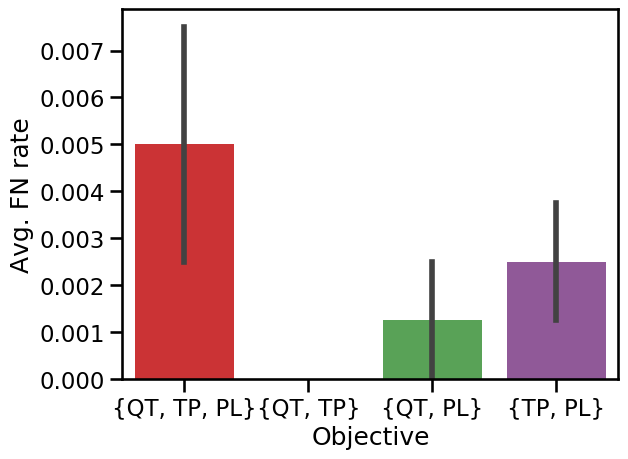
\includegraphics[width=\textwidth]{Figure/11-taxon_obj_wise_perf}
		\caption{11-taxon}
\end{subfigure}\begin{subfigure}[b]{0.33\textwidth}
		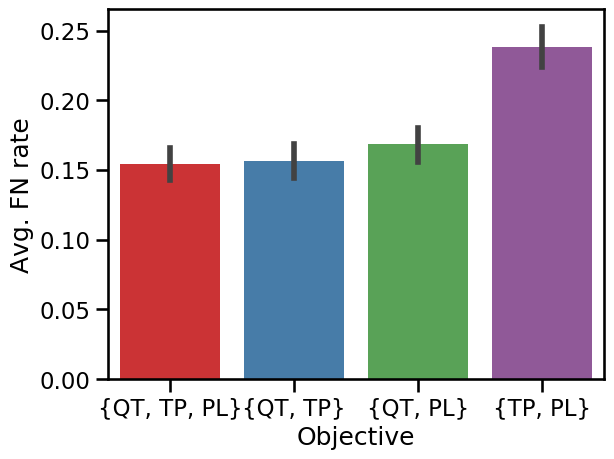
\includegraphics[width=\textwidth]{Figure/15-taxon_obj_wise_perf}
		\caption{15-taxon}
\end{subfigure}
	\caption{Variation of HV with generations for NSGAII and SNOGA on three datasets.}
	\label{fig:obj_wise_perf}
\end{figure*}


\begin{figure} [htbp]
\centering
	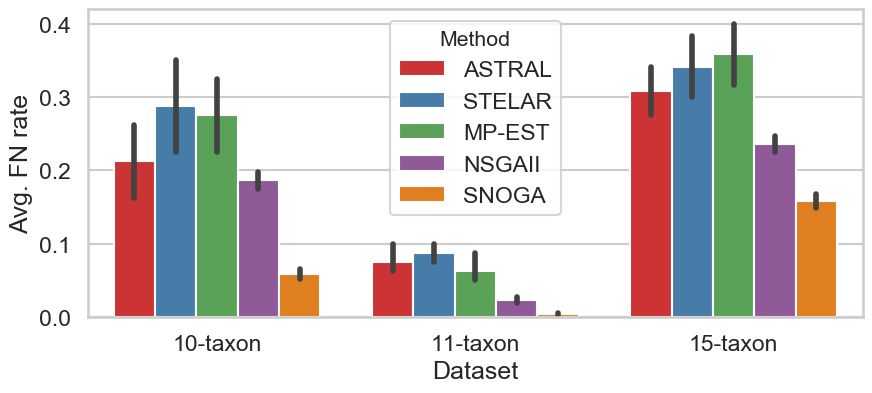
\includegraphics[width=0.7\textwidth]{Figure/all_dataset_compare}
	\caption{Performance comparison of ASTRAL, STELAR, MP-EST, NSGAII and SNOGA on three datasets. 
} \label{fig:compare_exisitng_methods}
\end{figure}
\subsection{Comparison with Existing Methods}
Finally, we evaluated the best trees offered by NSGAII and SNOGA in comparison with the output of ASTRAL, MP-EST and STELAR. On each dataset, we ran both NSGAII and SNOGA only for 99 generations (population size: 100, function evaluations: 10000). 
Fig.~\ref{fig:compare_exisitng_methods} shows the average FN rates with standard error bars over 10 replicates. We find that SNOGA offers the highest accuracy among all. On the 10-taxon dataset, SNOGA can achieve nearly 4X accuracy than ASTRAL. For the rest two datasets, the accuracy improvement is around 2X compared to ASTRAL. Interestingly, even the basic NSGAII exhibits more accuracy than the three existing methods. So the advantage of formulating this problem as a MOP is obvious. From actual application point of view, if we run the original NSGAII algorithm for a large number of generations its accuracy may fall for not resolving the issues mentioned in Section~\ref{sec:problem} properly which we saw earlier. Note that the FN rate is not the fitness criterion of the optimization process. Rather, the optimization continues based on the objective values.
So we can state that, owing to the characteristics designed considering the problem nature, SNOGA achieves at least 1.4X accuracy gain over the original NSGAII in all datasets. 





\begin{comment}
\begin{figure}[!htbp]
\centering
\begin{adjustwidth}{-1cm}{}
\begin{subfigure}[b]{0.55\textwidth}
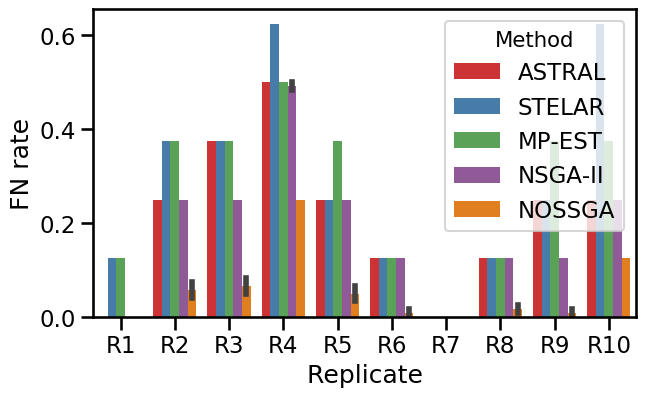
\includegraphics[width=\textwidth]{Figure/10-taxon_10_replicates}
\caption{10-taxon}
\end{subfigure}\begin{subfigure}[b]{0.55\textwidth}
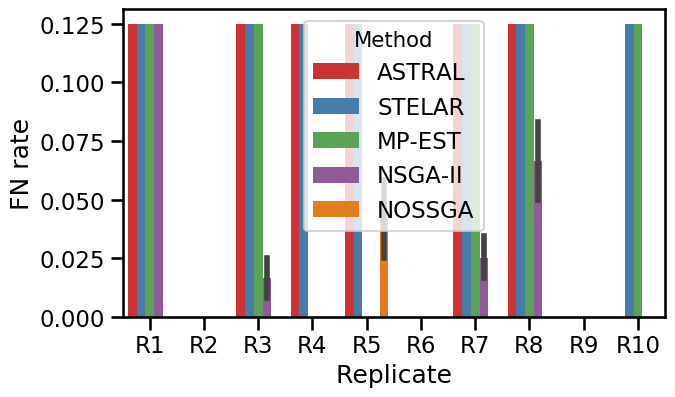
\includegraphics[width=\textwidth]{Figure/11-taxon_10_replicates}
\caption{11-taxon}
\end{subfigure}

\begin{subfigure}[b]{0.55\textwidth}
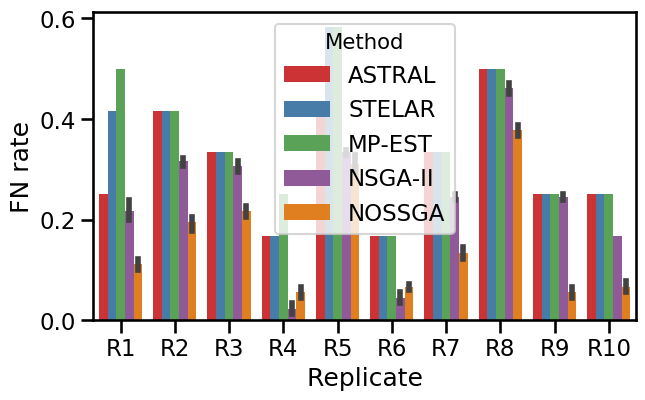
\includegraphics[width=\textwidth]{Figure/15-taxon_10_replicates}
\caption{15-taxon}
\end{subfigure}
\begin{subfigure}[b]{0.55\textwidth}
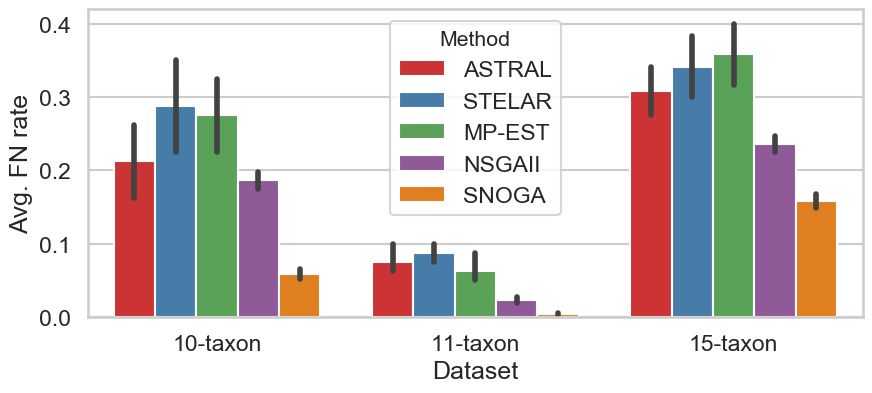
\includegraphics[width=\textwidth]{Figure/all_dataset_compare}
\caption{Summary}
\end{subfigure}

\caption{Comparison of ASTRAL, STELAR, MP-EST, NSGAII and SNOGA on 10 replicates of 3 datasets.}
\label{fig:datasets}
\end{adjustwidth}
\end{figure}



\begin{figure}[!htbp]
\centering
\begin{adjustwidth}{-1cm}{}
\begin{subfigure}[b]{0.48\textwidth}
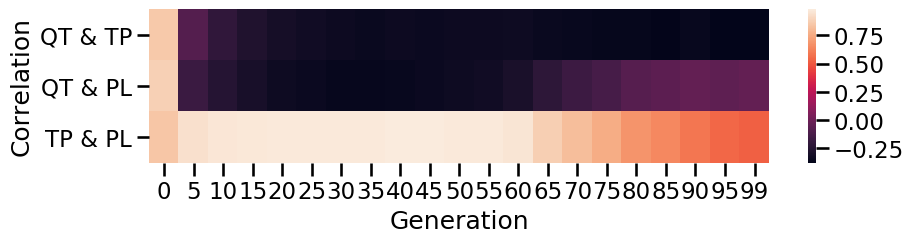
\includegraphics[width=\textwidth]{Figure/10-taxon_NSGA-II_heatmap}
\caption{NSGAII: 10-taxon}
\end{subfigure}\begin{subfigure}[b]{0.4\textwidth}
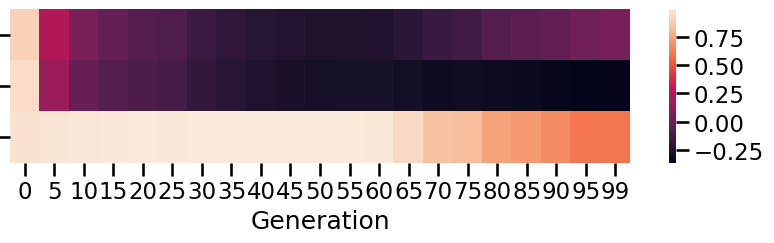
\includegraphics[width=\textwidth]{Figure/11-taxon_NSGA-II_heatmap}
\caption{NSGAII: 11-taxon}
\end{subfigure}\begin{subfigure}[b]{0.4\textwidth}
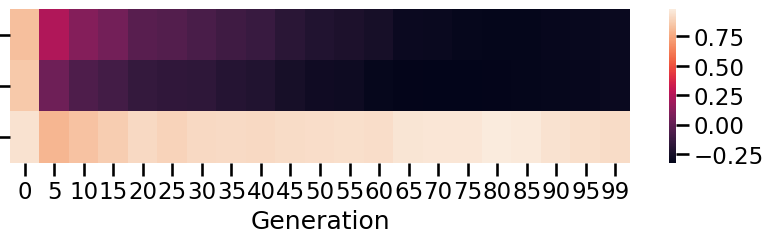
\includegraphics[width=\textwidth]{Figure/15-taxon_NSGA-II_heatmap}
\caption{NSGAII: 15-taxon}
\end{subfigure}

\begin{subfigure}[b]{0.48\textwidth}
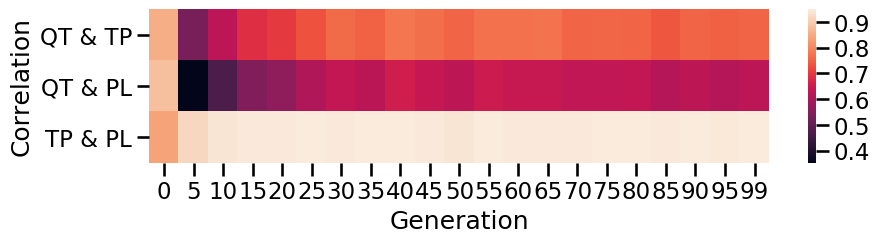
\includegraphics[width=\textwidth]{Figure/10-taxon_NOSSGA_heatmap}
\caption{SNOGA: 10-taxon}
\end{subfigure}\begin{subfigure}[b]{0.4\textwidth}
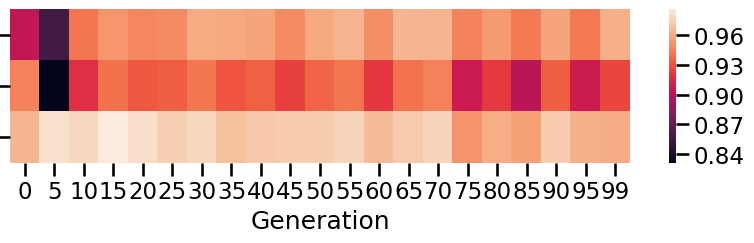
\includegraphics[width=\textwidth]{Figure/11-taxon_NOSSGA_heatmap}
\caption{SNOGA: 11-taxon}
\end{subfigure}\begin{subfigure}[b]{0.4\textwidth}
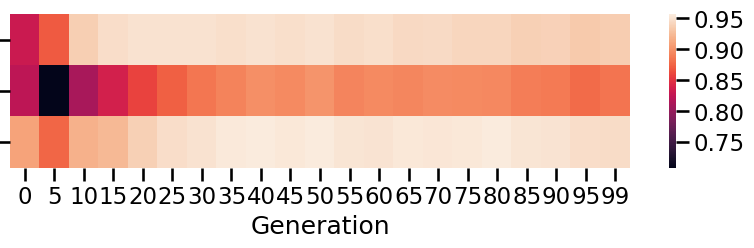
\includegraphics[width=\textwidth]{Figure/15-taxon_NOSSGA_heatmap}
\caption{SNOGA: 15-taxon}
\end{subfigure}
\caption{Correlation between each pair of objectives as the generation of an EMO progresses. For each dataset, we average the correlation coefficient over 15 runs and 10 replicates.}
\label{fig:gen_wise_correlation}
\end{adjustwidth}
\end{figure}
\subsection{Results on 10-taxon dataset}
\subsection{Results on 11-taxon dataset}
\subsection{Results on 15-taxon dataset}
\end{comment}

 \section{Conclusion} In this paper, we have introduced the problem of estimating species trees from a set of gene trees as an MOP. We have shown examples where the existing method, optimizing a single criterion, can overshoot the criterion and thus deviate from the true species tree. We have selected three objectives from three existing methods. Unlike traditional MOPs, optimizing an objective beyond a certain limit and discarding a dominated solution at an early generation can reduce the chance of generating better trees. Hence we cannot expect PF, sampled by a classical EMO algorithm, to contain highly accurate trees. Therefore, we have designed a specialized EMO algorithm, namely, SNOGA, which is a modification of NSGAII. We have analyzed the behavioral difference between SNOGA and NSGAII on a collection of challenging simulated datasets and found that the best trees offered by SNOGA are much better than the best trees generated by NSGAII. Our results suggest that a Pareto dominance based EMO algorithm may not be appropriate for effectively solving this problem. We also provided empirical justification for incorporating multiple objectives. Finally, we have shown that the tree-space generated by SNOGA contains highly accurate trees in comparison with widely used methods that optimize a single criterion. 





We are currently working to devise a systematic methodology to filter a limited number of better trees from the final population without the knowledge of the true tree provided with the simulated dataset. At present, our mutation selects one from NNI/SPR/TBR at random with equal probability. As a future improvement, we will improve it by adaptively adjusting the selection probabilities based on the success rate of an operator in the previous generation. Also, we are planning to embed domain knowledge inside NNI, SPR and TBR so that they can make informed (as opposed to random) rearrangement in the given tree. To enable SNOGA processing large datasets within a reasonable time, we will improve the efficiency of objective evaluations. Moreover, we are adapting a popular decomposition based EMO algorithm, namely, MOEA/D~\cite{zhang2007moea}, to effectively solve this problem. 


